% !TeX root = ../thuthesis-example.tex

\chapter{THEORETICAL EVALUATION OF THE VR-IOT RESEARCH PLATFORM}

A theoretical assessment of the various parameters of the platform is provided in this chapter. Compared to the existing solutions on the market, this is the first solution to automatically add any device from the real world to Virtual reality. Also, the platform allows researchers to create new devices in Virtual reality through the Things designer. Even though this research's main goal was to design the platform, the API for external projects connected to the platform will be presented. The limitations dictated by hardware were considered in the previous chapter. In this chapter, the limitations dictated by the architecture are discussed.

A functional solution for IoT research requires support for various types of devices. Although the IoT market has tens of thousands of different devices, general types of device parameter values ​​can be specified. Following the definitions given in Chapter 3, each device is represented as a Thing and includes several Items. Thus, each device existing or created in the future can be divided into blocks in terms of the VR-IoT Research Platform architecture. The supported Item types are listed in the Table~\ref{tab:items-table}.

\begin{table}
  \centering
  \begin{threeparttable}[c]
    \caption{The supported Item types}
    \label{tab:items-table}
    \begin{tabular}{ll}
      \toprule
      ITEM TYPE    &         DESCRIPTION                 \\
      \midrule
      Color &	RGB Color value \\
      Contact & Whether the sensors are located close enough to each other \\
      DateTime & Date and time parameters \\
      Dimmer &	Dimmer value in percentage \\
      Group &	An Item containing other Items \\
      Image &	The binary data of an image \\
      Location & GPS Coordinates \\
      Number & Value stored in number format \\
      Number:<dimension> & Number Item with specified unit support \\
      Player & Item that control video, audio playback \\
      String &	Text or binary data \\
      Switch & Boolean value \\
      \bottomrule
    \end{tabular}
  \end{threeparttable}
\end{table}

The universal Item data is String since the data collected by IoT sensors can be represented in binary format in almost all cases. Hence, the data operated by IoT devices can be placed inside Item blocks.

After NUIX-Studio App receives the Item of a specific format, the Semantic model is updated. Next, the Item corresponding Widgets are updated as well.

\section{Widgets support}

The platform provides only basic Widgets for the Items. These Widgets are used to give an example of how to visualize the IoT devices' data. Researchers can create Widgets specific to the device they develop using the NUIX-Studio API.

However, in most cases, researchers can save time by using the basic Widgets. Several Widgets based on the Mixed Reality Toolkit (\cite{MRTK2021}), such as Color Picker, Pinch Slider, Switcher, and Button, were developed. Light-connected, Player-, Location- and Group-based Widgets were developed without using Mixed Reality Toolkit.

\section{Things designer}

Thanks to using a block structure to represent devices, researchers can change various parameters of existing devices by changing specific blocks and create new devices by combining the blocks. This action is possible in a tool called Things designer. Further, this tool is described in detail.

The Semantic model is visualized inside the Web interface. Researchers can assign Widgets for each of the Items and group the Items. After the setup is completed, researchers can further develop new devices inside the NUIX-Studio App. Next, they can create new Widgets inside VR and connect them to the existing Items. The position for each of the Widgets is added to the Semantic model as an Item. Having set the widget's position and other parameters, the user can exit the application on a device and then continue research using a different device or analyze the items' data stored on the server. Since changes in Items values are periodically written to the server, they can be visualized by the built-in system tools (Figure~\ref{fig:PersistenceExample-figure}) or further analyzed using external frameworks providing useful insights. In addition, NUIX-Studio App also allows the creation of not only Widgets but also Items. However, this functionality is limited at the moment, but, in theory, it will be possible to develop any device with support for creating Items for all types of data.

\begin{figure}
  \centering
  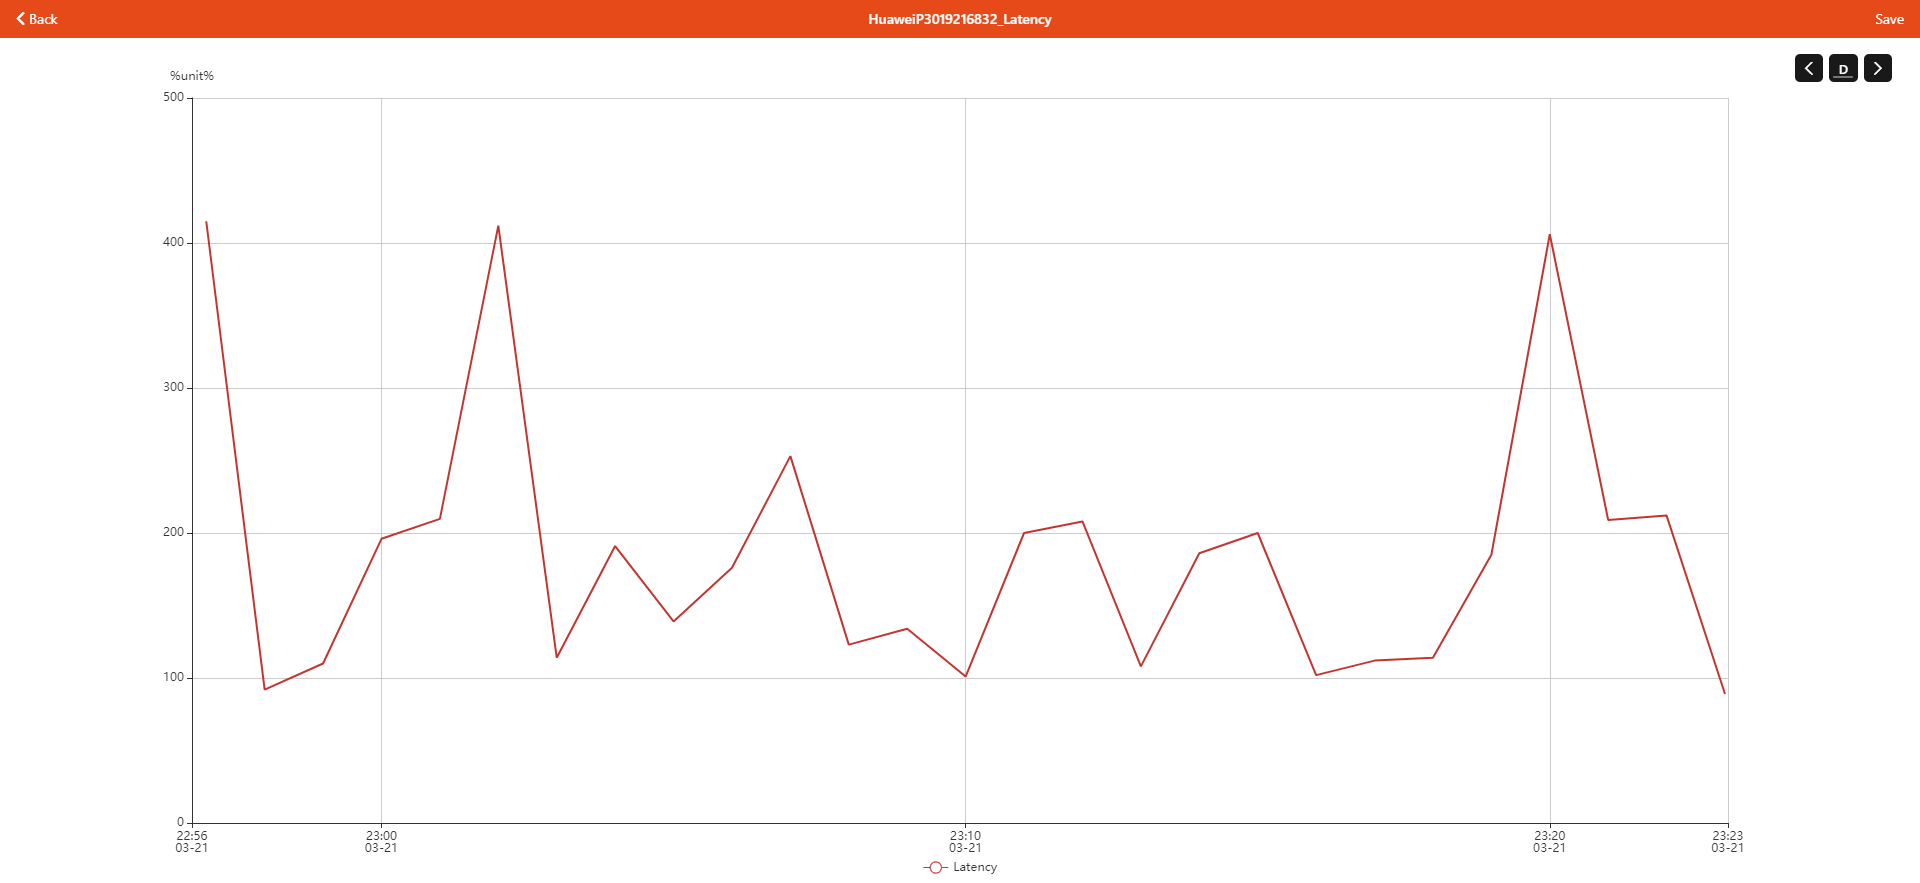
\includegraphics[width=0.9\linewidth]{figures/PersistenceExample.png}
  \caption{Persistence example: Latency value for accessing a remote device (in ms). }
  \label{fig:PersistenceExample-figure}
\end{figure}

\section{Device visualization and real-virtual world location mapping}

Each of the IoT devices is visualized through Widgets, but Widgets' designing by 3D modeling requires additional time. If a 3D model of the device already exists, the researcher can add it to the platform as a Widget and then connect extra widgets to it.

But very often, when developing new devices, a 3D model of the device has not yet been created, or in the used IoT environment, many devices also do not yet have the corresponding 3D models. There are several solutions to this problem. The first solution is to use 3D models of similar devices. However, it is not always possible to find the particular model, or the quality of these models does not meet the requirements. The second solution is device scanning. With the help of 3D scanners based on depth cameras, it is already possible to scan things with acceptable accuracy, especially at a relatively affordable price. If millimeter precision scanning is required, then expensive professional solutions can be used.

The resulting Widgets of 3D models are added to virtual reality. In the case of the NUIX-Studio App, scenes representing different environments are used. An example scene is demonstrating a smart home environment. Scenes can be created within Unity editor and using Things designer by interpreting the surrounding objects as Widgets (for example, people's position on the street is represented as an Item of Location type). This approach takes quite a long time to construct a scene, especially if there is a need to use a copy of the real environment in Virtual reality. To reduce the simulation time, researchers can use solutions such as 3D scanning the environment. It is possible to scan the environment with good accuracy on many different smartphones using Depth Lab from Google and with excellent accuracy on the iPhone 12 Pro using Apple ARKit. However, these scans of the environment are static scenes. If an object inside this environment is moved, then the scan will have to be performed again. Unfortunately, there is currently no solution to this problem. However, in the next chapter, it will be shown that the platform can be adapted to work with augmented reality, thus eliminating the need to match the real world with the virtual one fully.

Various devices can track the movement of real IoT devices in the real world, such as Bluetooth tags, QR codes, magnetic field sensors, etc. Researchers can use API to change the position of each widget. Thus, when the device's position in the real world changes, the device's Widgets position in the virtual world will also change. Besides, it is possible to perform the opposite action, but this requires a device that will move IoT devices in the real world.

\section{Physics support}

With the transfer of resource-intensive calculations to a separate server, it becomes possible to perform more reliable physical object simulations. Computations such as processing light, sound, and electromagnetic waves of other frequencies and various substances such as gas, water, are only limited by existing algorithms.

\section{Scalability}

When the number of Widgets within the system increases, platform performance remains at an acceptable level. Because each Widget is assigned some unique id, the time it takes to access a specific Widget is O(1) operations. Event processing time takes O(n) operations, where n is the number of connected widgets. It is theoretically impossible to reduce the complexity of processing an event since every Widget has to be accessed. In this case, the event processing time is linearly dependent on the number of Widgets connected to the Item. In general, the platform's overall performance also linearly depends on the number of IoT devices in the environment.

\section{Conclusion}

Thus, it was shown that the platform's architecture allows support of all possible devices, creation of new devices from existing ones, and placing them in the virtual world. The platform enables the efficient processing of requests from an unlimited number of devices.

However, the platform's architecture does not circumvent the limitations associated with some theoretical calculations. Yet, in order to get around these limitations, researchers can use the platform inside Augmented reality, which is discussed in more detail in the next chapter.